\documentclass{ximera}

\author{Wim Obbels and Bart Snapp}

\title{First steps in Ximera}

\begin{document}
\pdfOnly{\onecolumn\begin{multicols}{2}}
        \begin{abstract}
            Try out Ximera!
        \end{abstract}
        \maketitle

        To use Ximera, you must have a \link[GitHub]{https://github.com}
        account. GitHub is a web platform where developers can store, share,
        and manage
        their code. It uses \verb!git!, popular software for version control,
        to help
        teams work together simultaneously without overwriting each other's
        changes.
        GitHub has
        \begin{itemize}
            \item issue tracking,
            \item pull requests for proposing changes,
            \item the ability to merge code,
        \end{itemize}
        and other project management tools. It's like a shared folder for
        coding, designed to
        help teams work together and track progress. Go to
        \url{https://github.com} and
        either \textbf{sign-up} or \textbf{log-in}. Note, you must know your \textbf{username}
        and
        \textbf{password}, so store them in a safe place; like in a safe, or
        under your
        bed. After you have a GitHub account, log-in and go to:
        \begin{center}
            \url{https://github.com/ximeraProject/ximeraFirstSteps}
            %% 230% on my horiz screen
        \end{center}
        You will see something like this:
        \pdfOnly{\end{multicols}}\enlargethispage{1.5em}
\begin{image}
    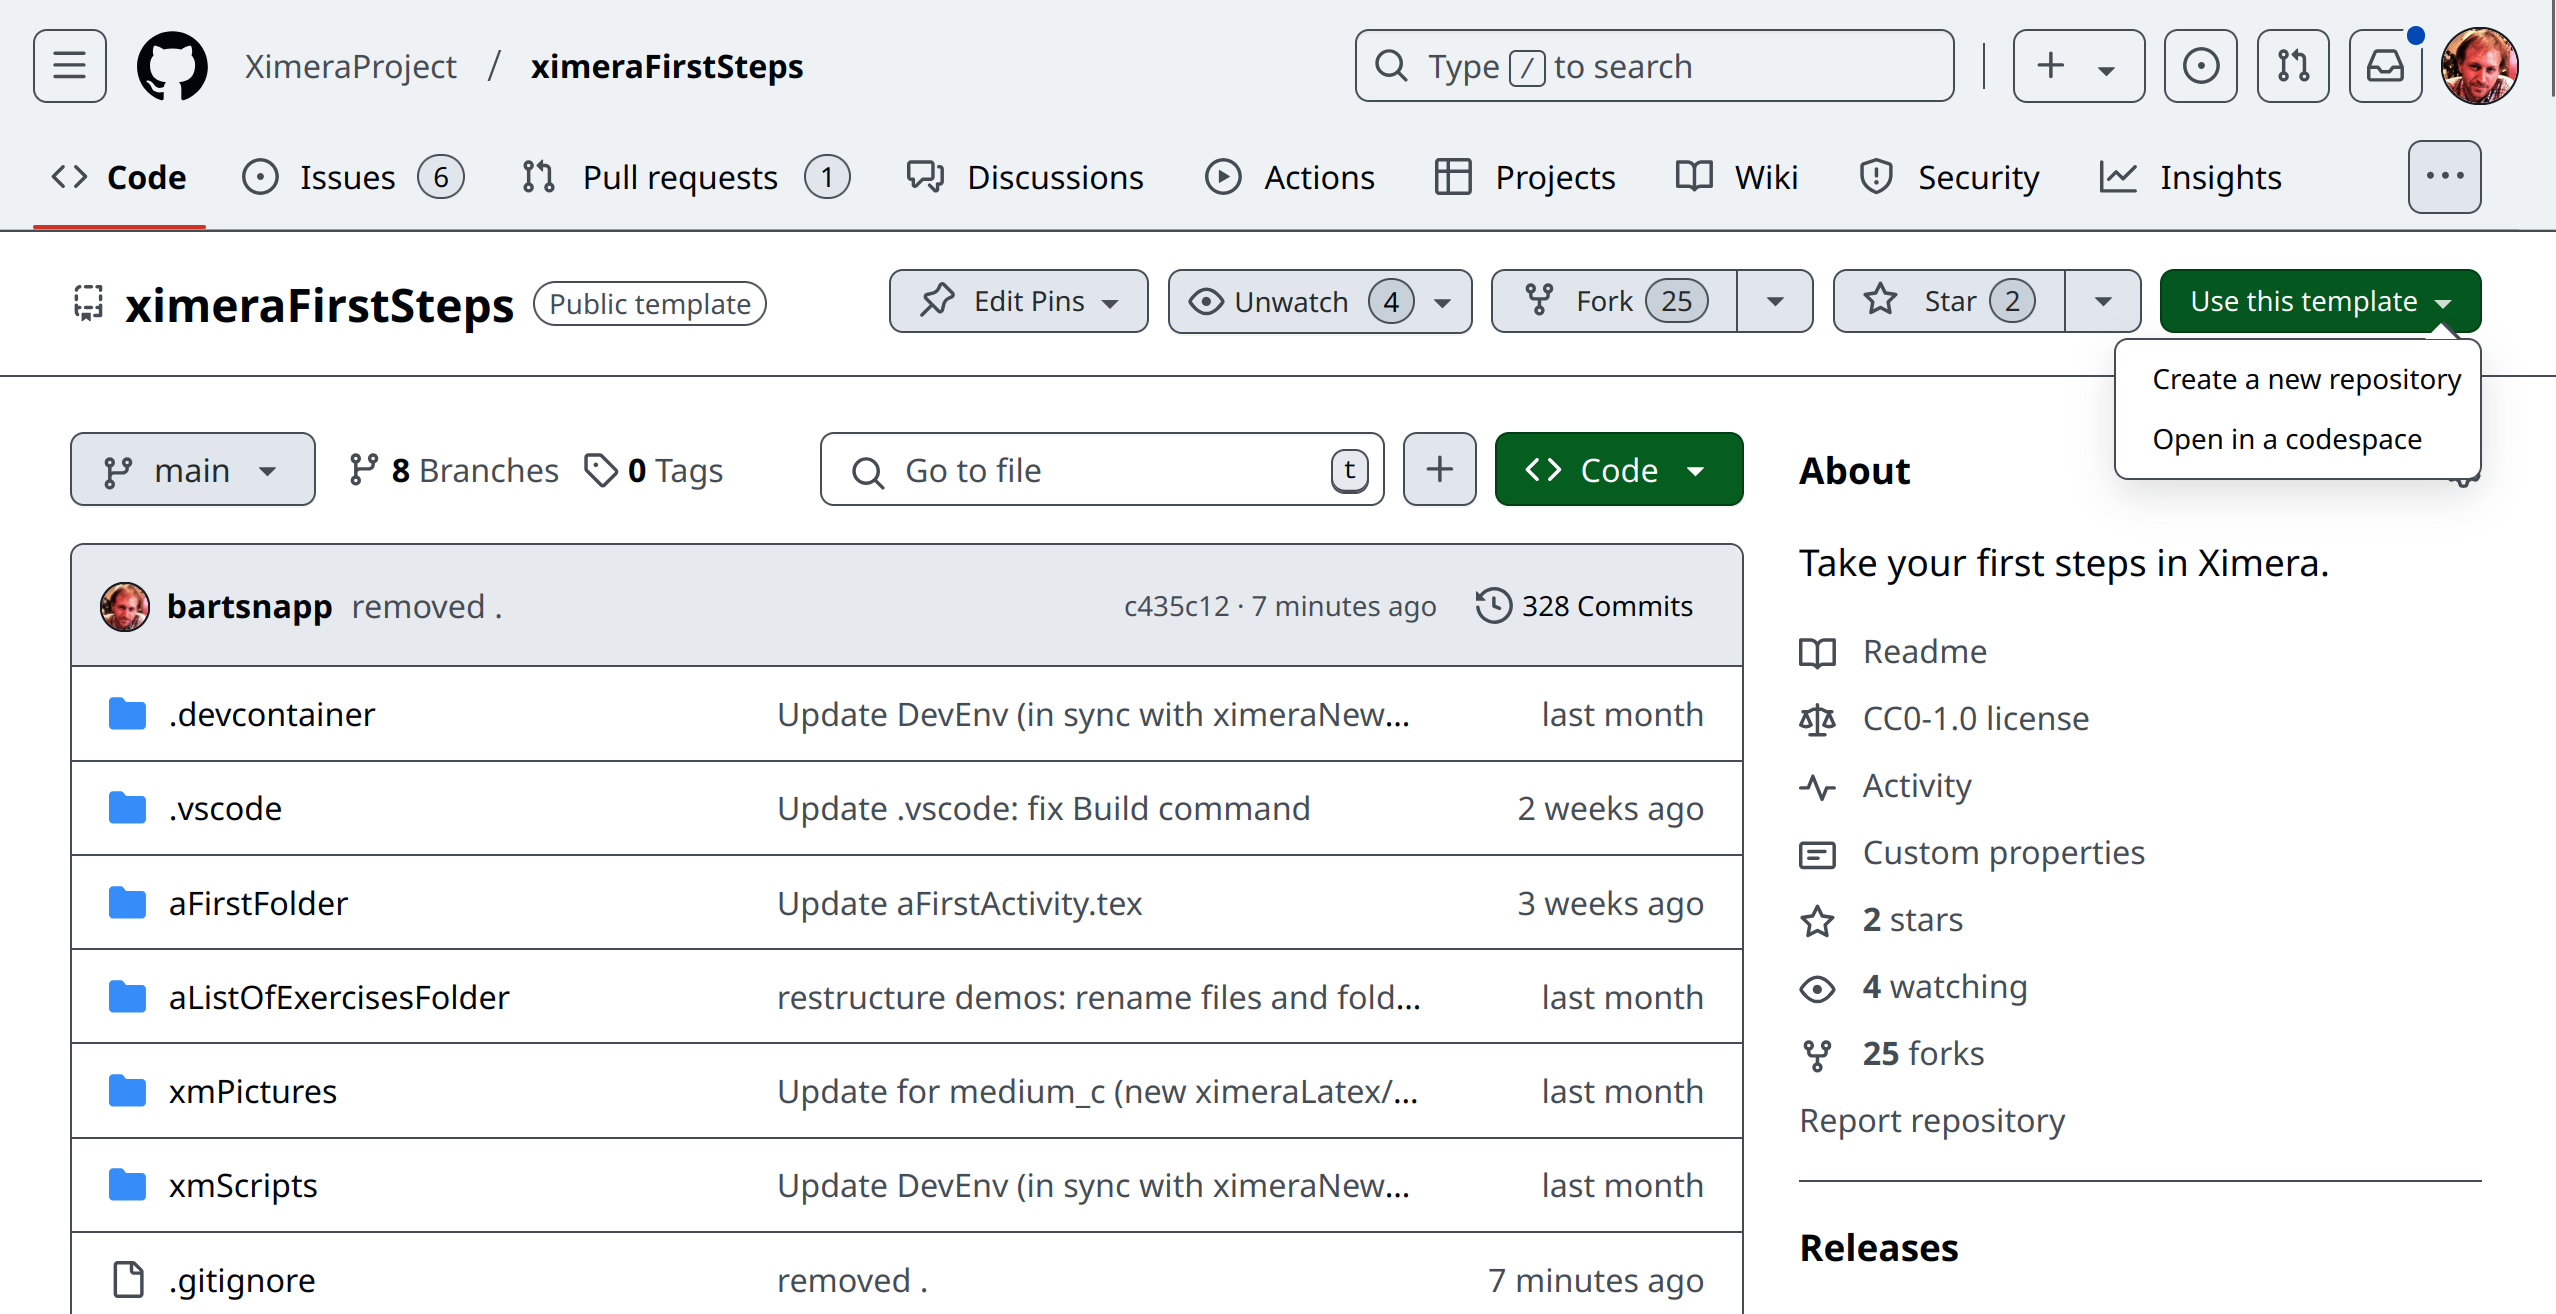
\includegraphics[width=.7\textwidth]{xfsTemplate}
\end{image}
\newpage

\begin{image}
    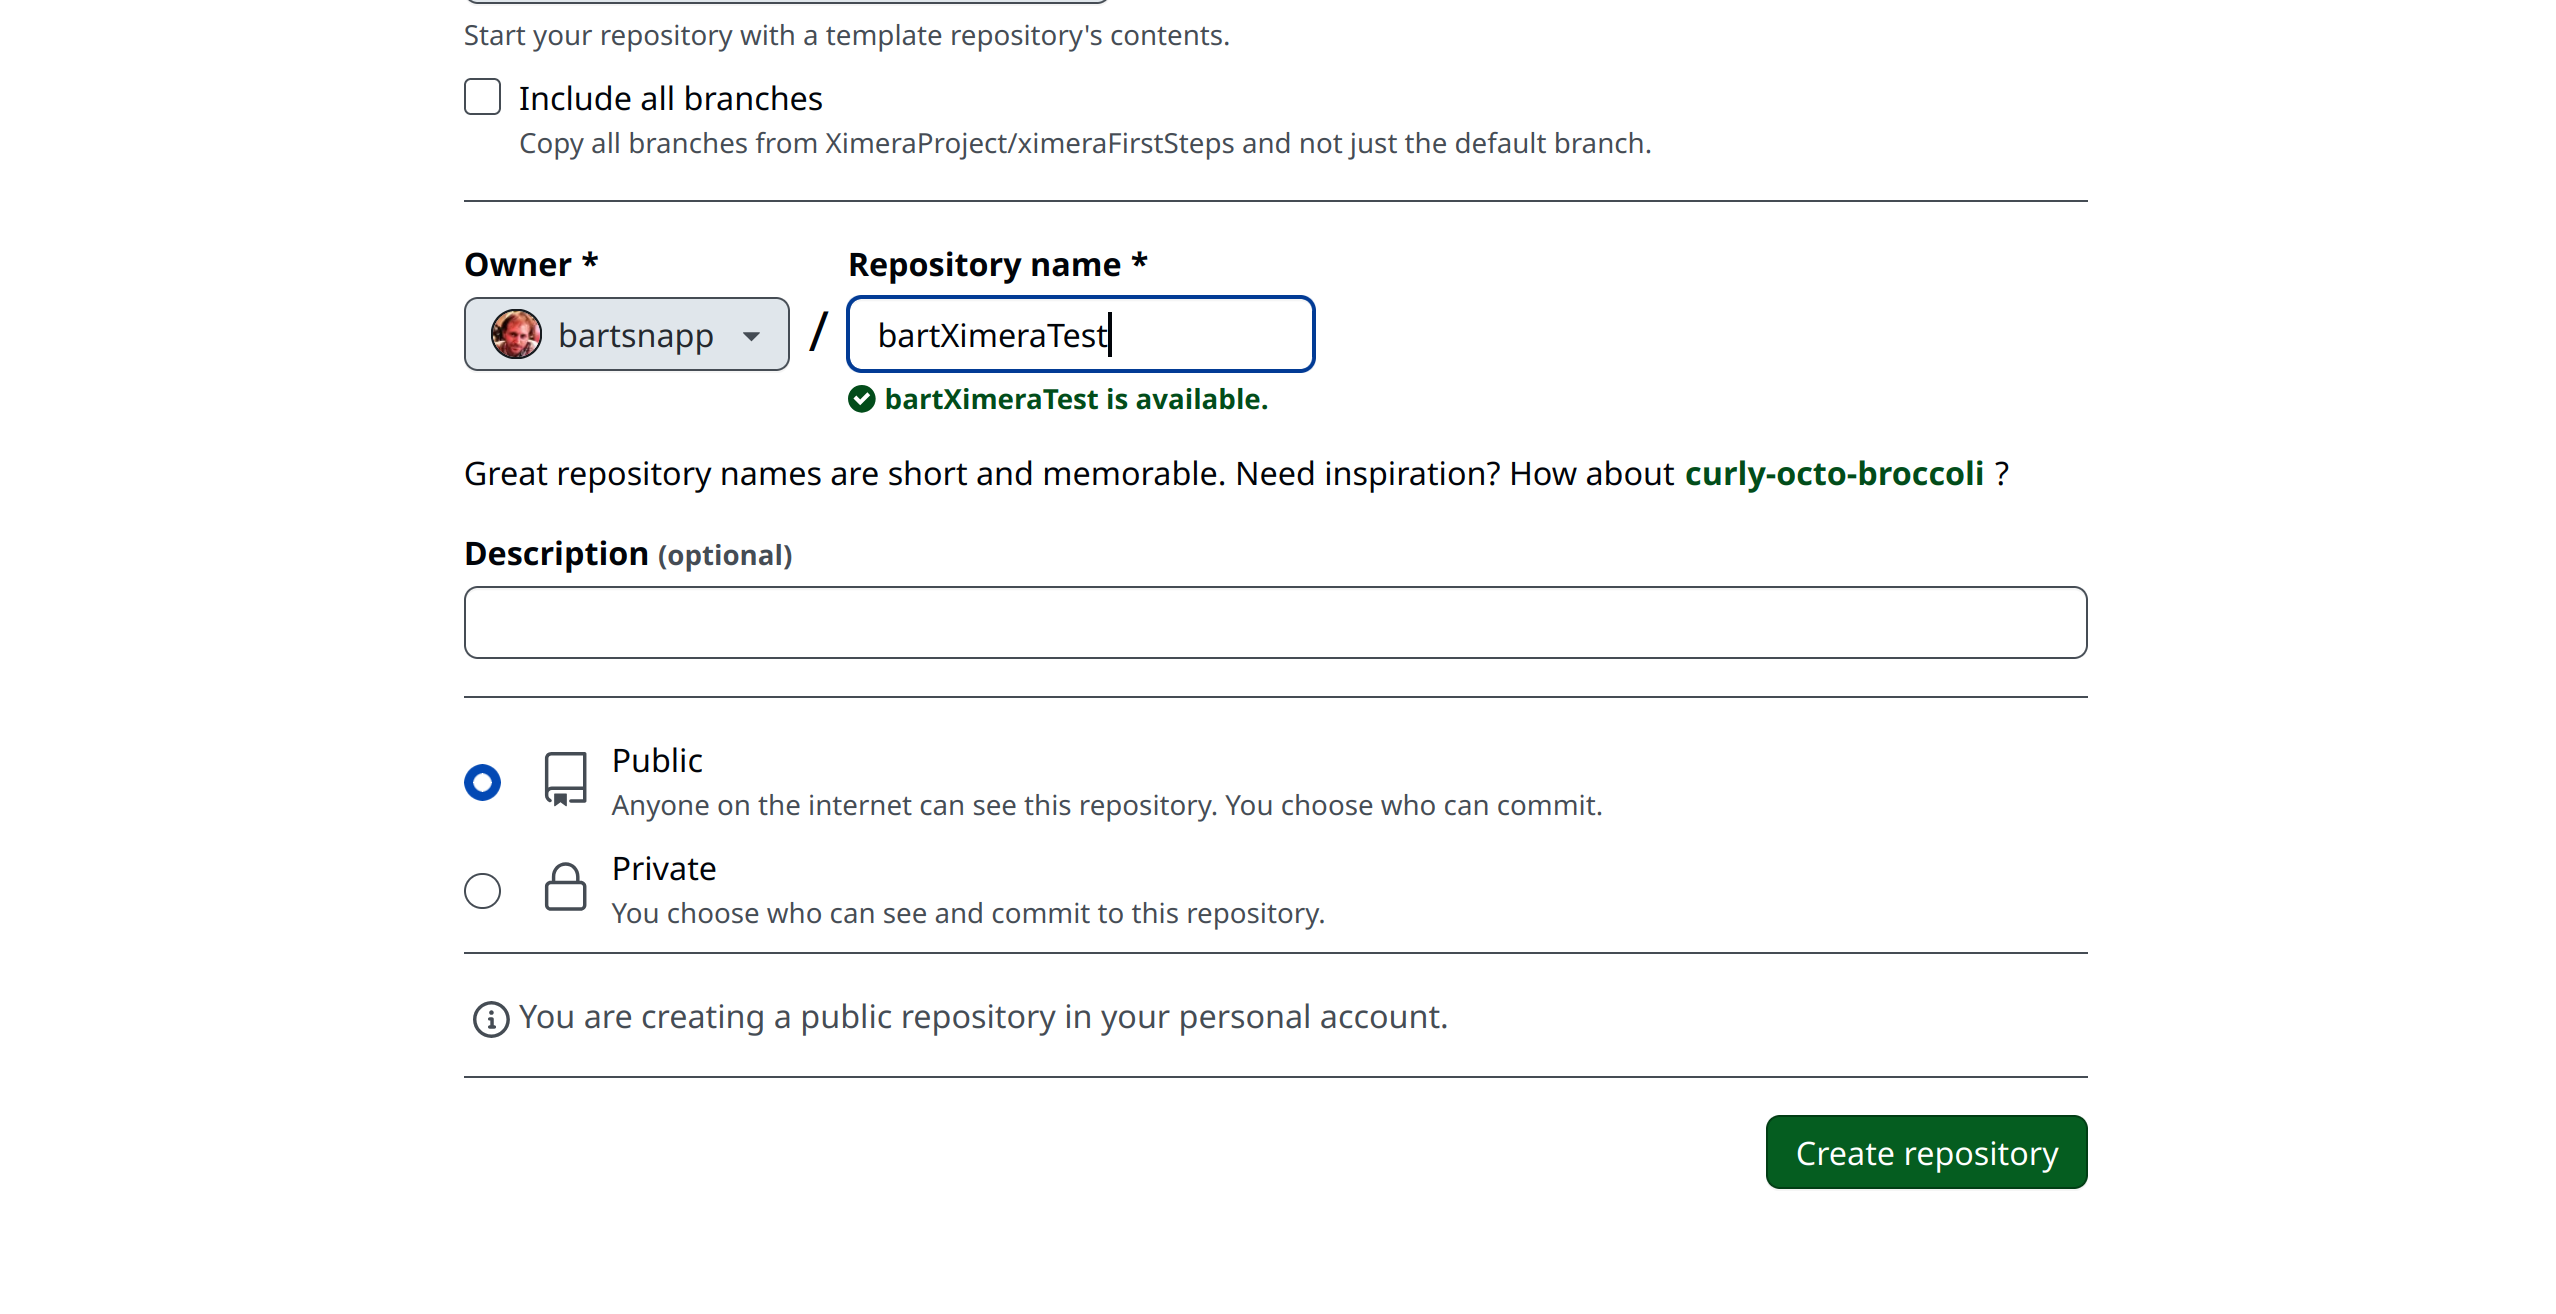
\includegraphics[width=.7\textwidth]{xfsCreate}
\end{image}
\pdfOnly{\begin{multicols}{2}}
        Click on the green ``Use this template'' button and select ``Create a
        new repository.'' Give it a fun repository name, and push the button
        ``Create repository.''
        At this point you have your own personal copy of our repository
        \verb!ximeraFirstSteps!.
        In fact, after you create it, GitHub will take you to it. This copy can
        always
        be found at:
        \begin{center}
            \verb!https://github.com/YOUR-GIT-USER-NAME/YOUR-REPO-NAME!
        \end{center}
        For the example used in this manual, the URL would be: 
        \begin{center}
            \verb!https://github.com/bartsnapp/bartXimeraTest!
        \end{center}
        \newpage
        \pdfOnly{\end{multicols}}
\begin{image}
    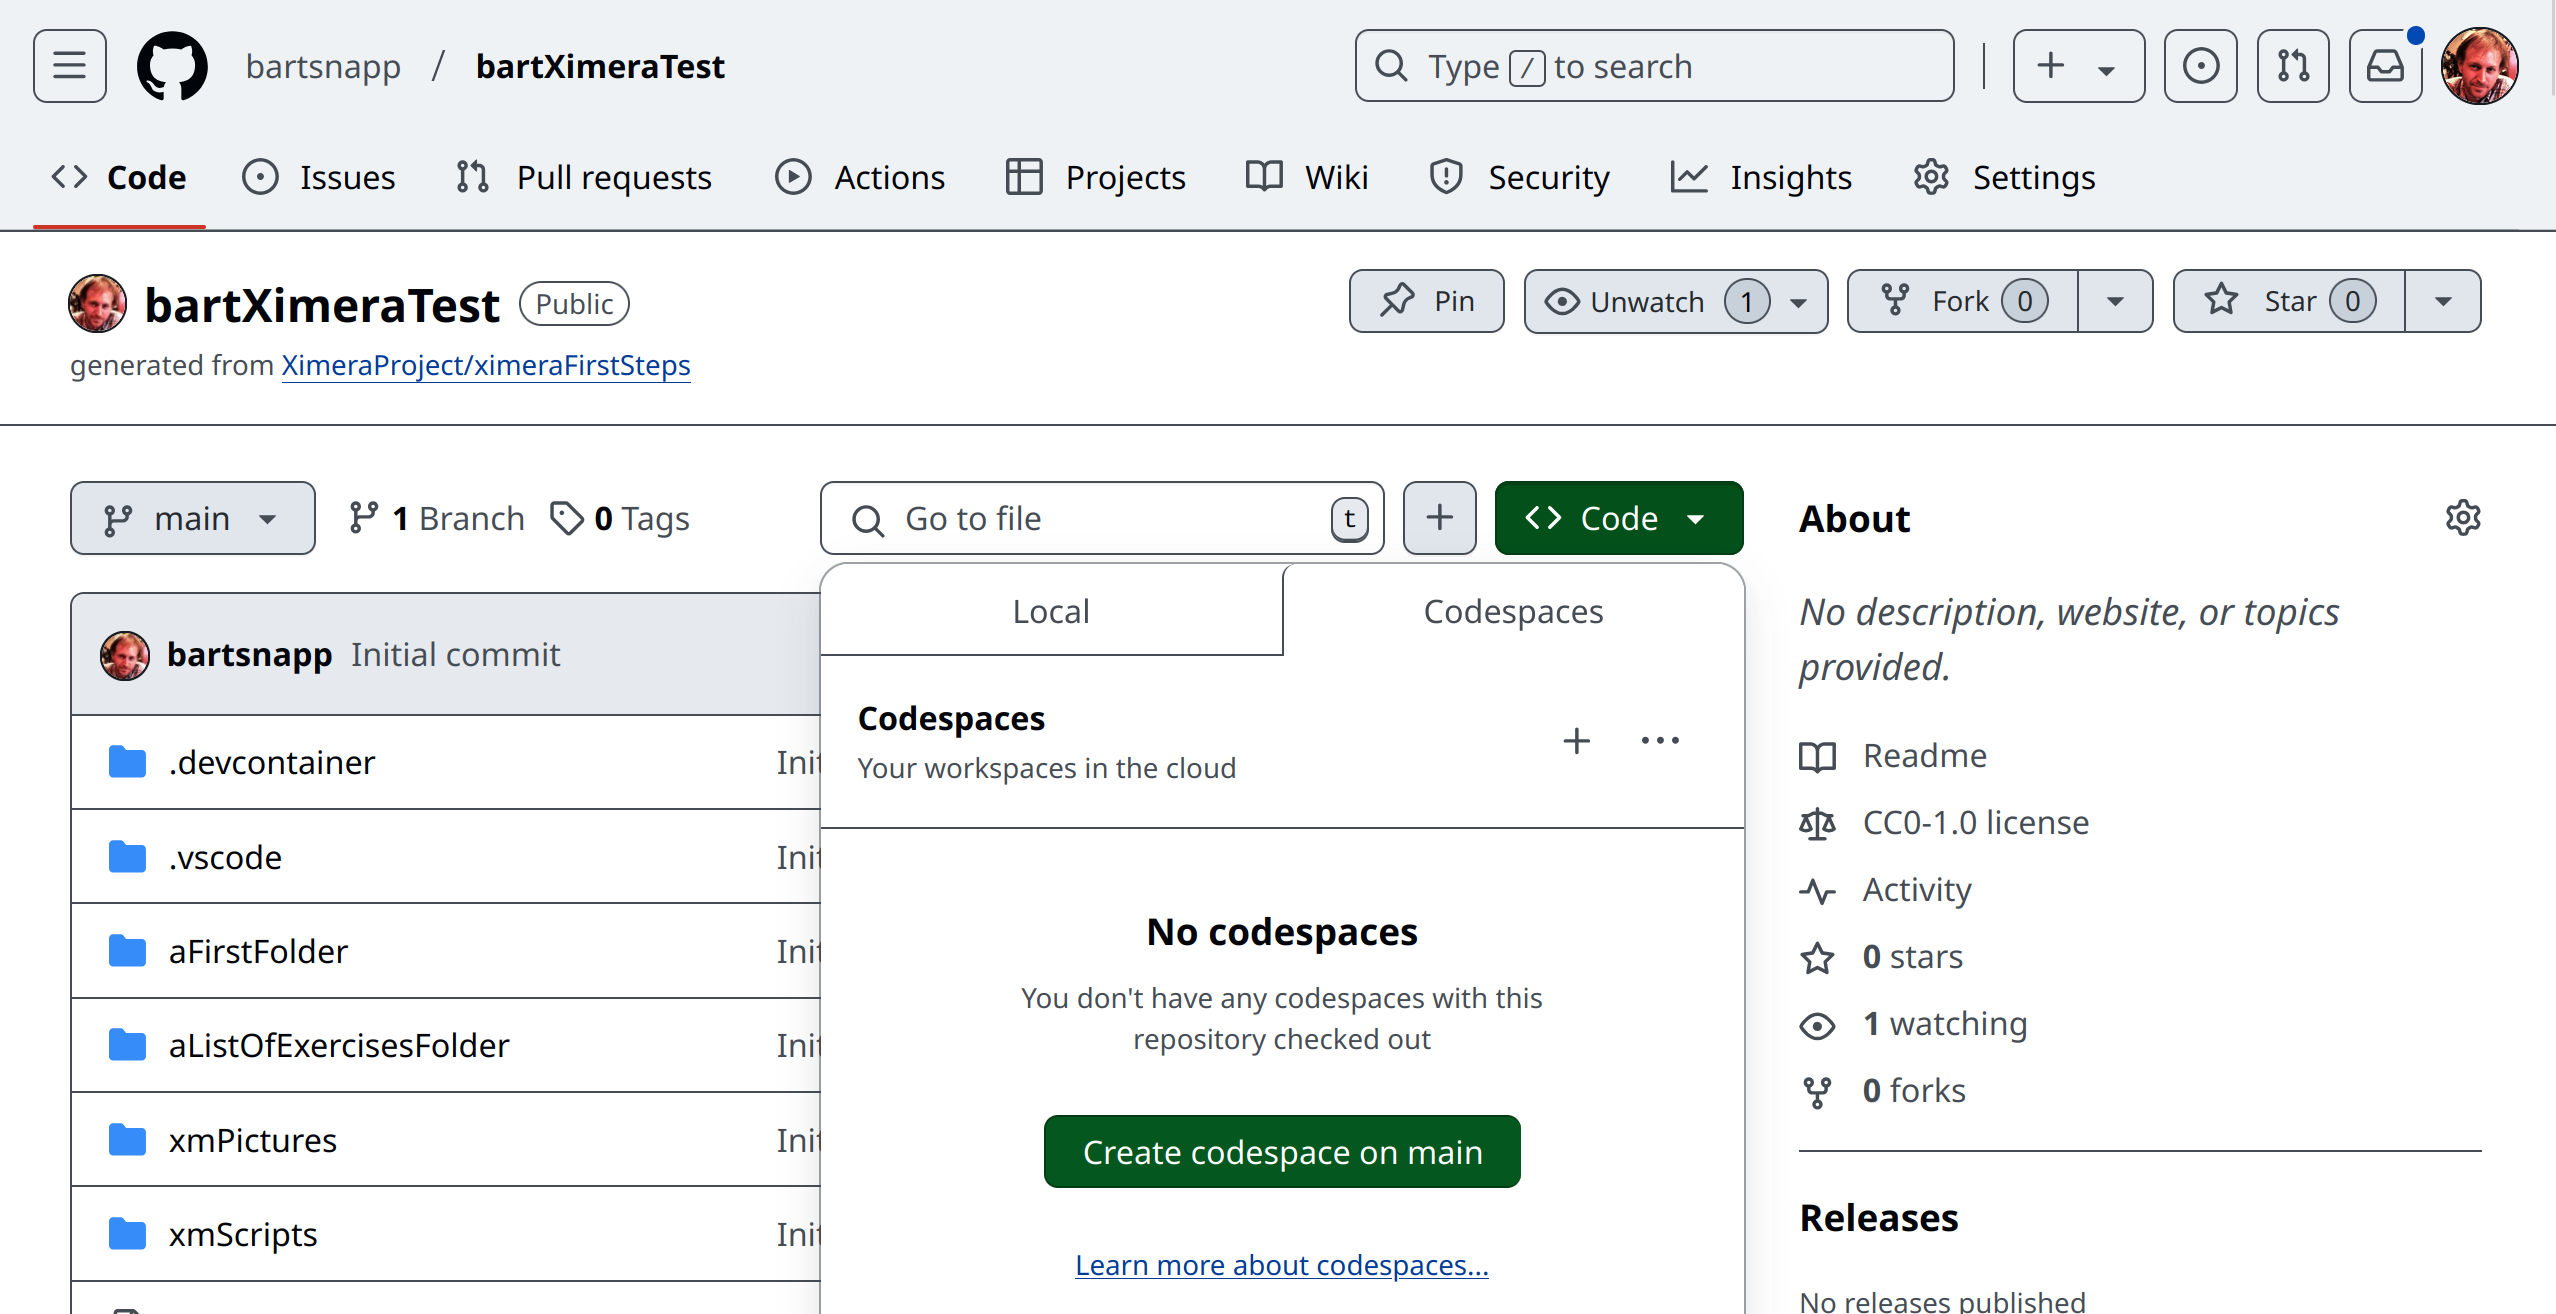
\includegraphics[width=.7\textwidth]{xfsCodespace}
\end{image}
\pdfOnly{\begin{multicols*}{2}}
        When at your repository, click the green ``Code'' button, select the ``Codespaces''
        tab, and click ``Create codespace on main.'' A GitHub codespace is a remote computer set up
        specifically for
        coding. \textbf{It will take
            around 5
            minutes for your codespace to be created and you must wait until it
            is
            complete.} We have our codespace preconfigured with all the tools,
        libraries, and
        software you need to use Ximera. With a codespace, you can instantly
        start
        working without worrying about setting up software on your local
        machine.
        Moreover, \textbf{Ximera developers} can go to your GitHub page, start
        their
        own codespace, and try out your code and directly help with possible issues.

        \pdfOnly{\end{multicols*}}

\newpage

\begin{image}
    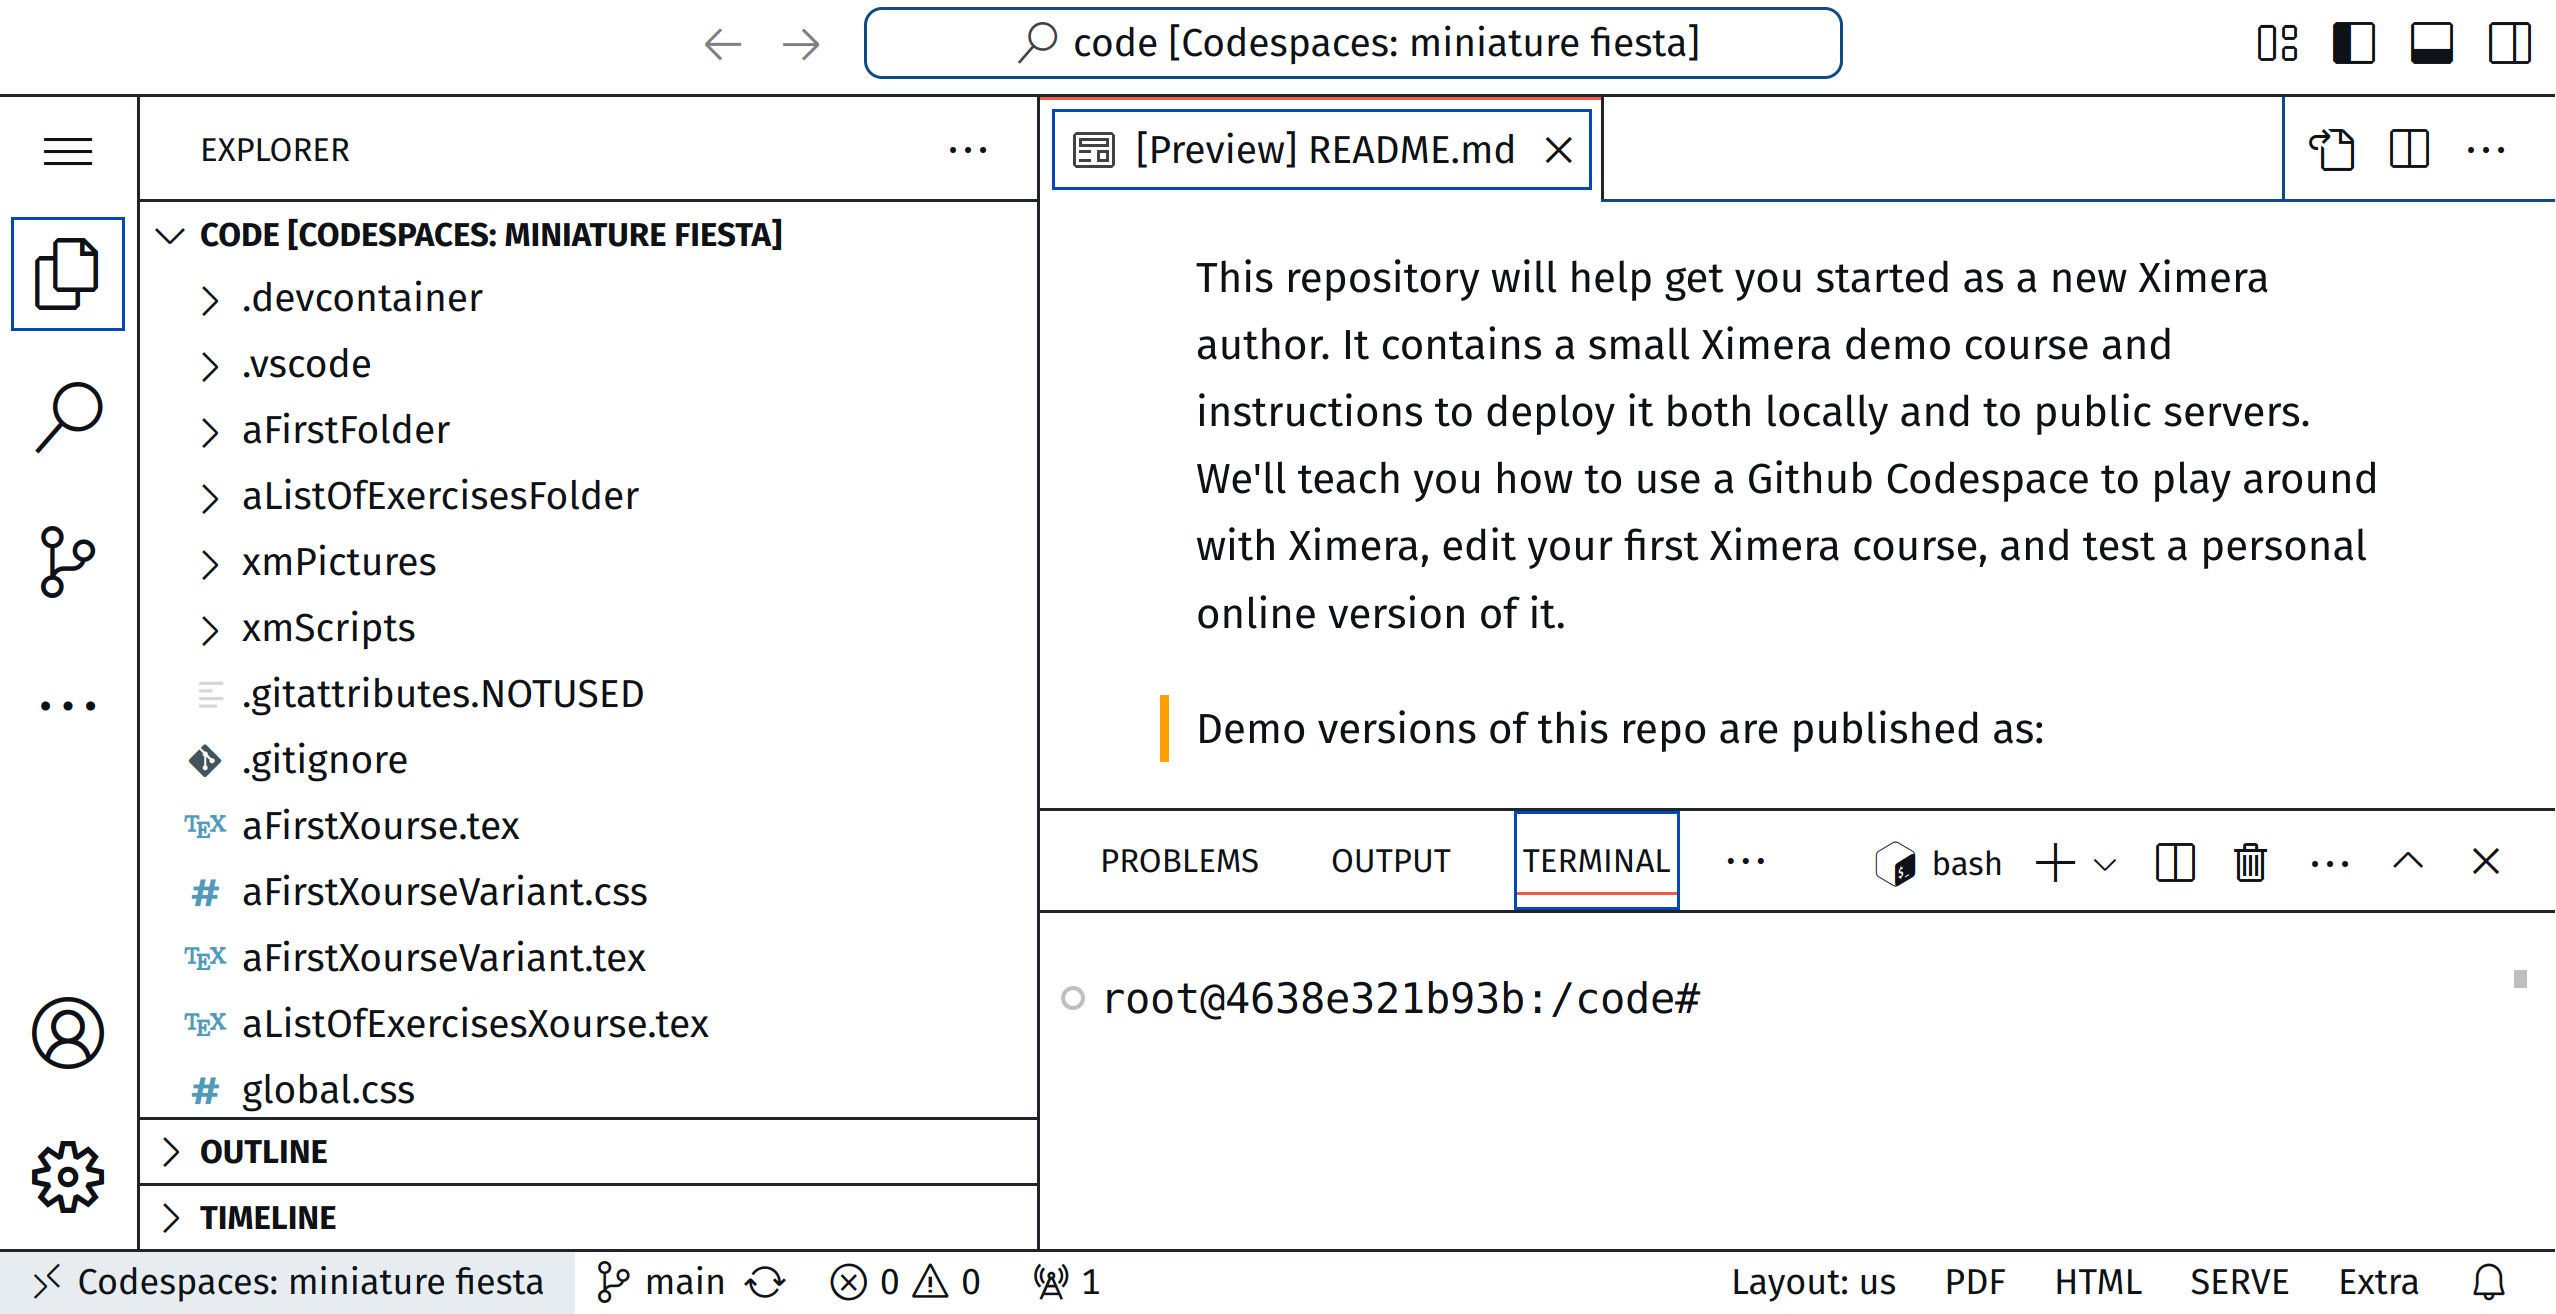
\includegraphics[width=.7\textwidth]{xfsVScode}
\end{image}
\pdfOnly{\begin{multicols*}{2}}
        Once the codespace is created, you will see something like what we have
        above. This is Visual Studio Code (VS Code) running within your browser. VS Code
        is a powerful text-editor with many extensions. We use it write Ximera content.
        On the far left, you see a vertical list of icons. Currently, ``EXPLORER'' is
        selected, it looks like ``pages of paper.'' Moving right, we see the files in
        our GitHub repository. At the bottom right-hand corner of the screen you will see
        buttons that say ``SERVE,''  ``HTML,'' and ``PDF.'' These buttons were added by the files
        in the hidden folder \verb!.vscode/!.
        \begin{description}
            \item[The ``SERVE'' button] compiles the \textbf{entire} Ximera repository to HTML and deploys to a (local or remote) server. If this is the first time you are compiling, it will take a few minutes.
        \item[The ``HTML'' button] compiles only the \textbf{current} \LaTeX\ file to HTML.
        \item[The ``PDF'' button] compiles only the \textbf{current} \LaTeX\ file to PDF using our Ximera tools.
        \end{description}
        At this point, you will want to press the```SERVE'' button. This will
        compile the entire repository and deploy it to a local server. As part of this process, 
        we will generate a GPG Key, that we use to help sign content online. 
        If you are simply playing with Ximera, you can just hit ``enter'' \textit{twice}.



        We will discuss deploying Ximera content to the open web in a later section.
        
        \pdfOnly{\end{multicols*}}

\newpage

\begin{image}
    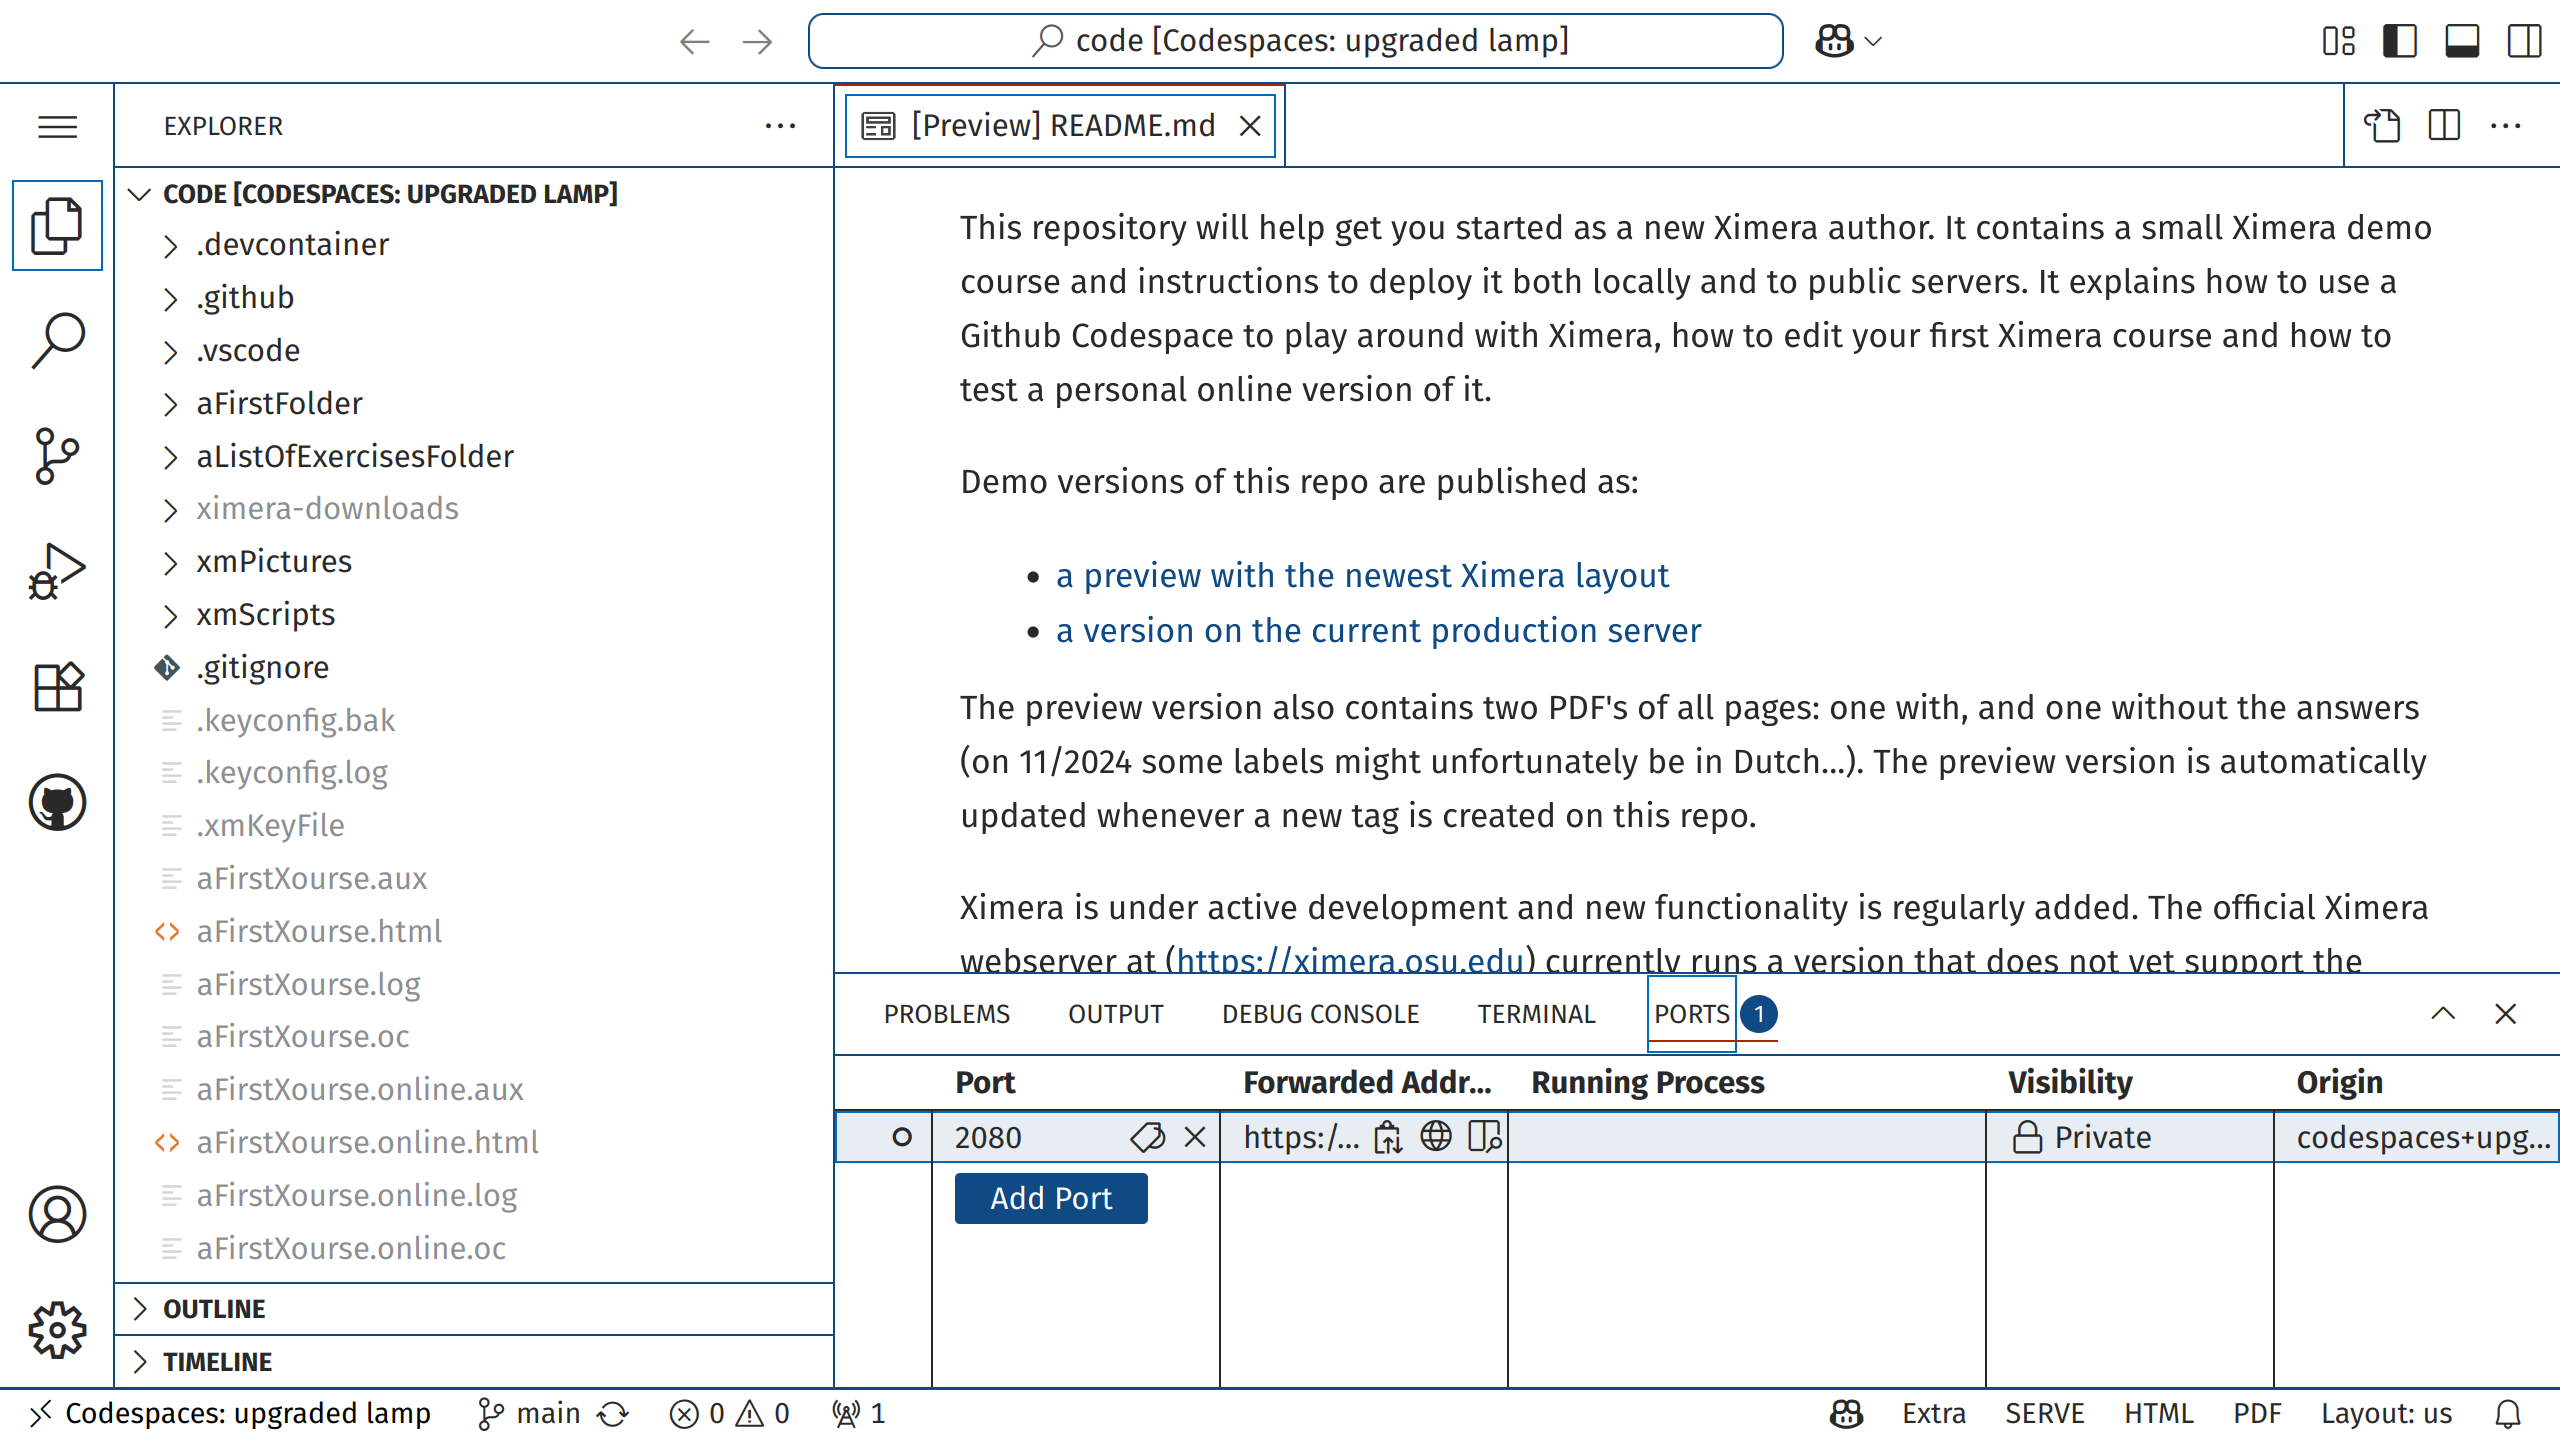
\includegraphics[width=.7\textwidth]{xfsPorts}
\end{image}
\pdfOnly{\begin{multicols}{2}}

    After you have pressed the ``SERVE'' button, you will see a
        ``terminal'' window at the bottom of the screen. 
        note the line that says: ``PROBLEMS,'' ``OUTPUT,'' ``DEBUG CONSOLE,''
        ``TERMINAL,'' ``PORTS.''
        You want
        to click on ``PORTS.'' The ``PORTS'' tab may be hidden within
        ``$\cdots$.''
        After you click on ``PORTS,'' select 2080 and click on the globe, and a
        webpage
        will open. Your
        content will be under the link ``Content.'' You should be able to see
        the
        content in your browser.

        You may delete your codespace (you can simply recreate it) and others
        can come
        to your GitHub repository, start a codespace, and check out and compile
        your
        code.
        This is especially useful if a user runs into difficulty, as a Ximera
        developer
        can examine a users exact setup, and help resolve any issues.

        Demo versions of this repository are published as:
        \begin{itemize}
            \item \link[a preview with the newest Ximera layout]{https://set.kuleuven.be/voorkennis/firststeps24/aFirstXourseVariant/aFirstFolder/aFirstActivityVariant}
            \item \link[a version on the current production server]{https://ximera.osu.edu/firststeps24/aFirstXourse/aFirstFolder/aFirstActivity}
        \end{itemize}

        \pdfOnly{\end{multicols}}
\pdfOnly{\twocolumn}
\end{document}